\chapter{От магнетиков Изинга к жидкость--газовой критичности}

\lectureoverview{К переходу жидкость--газ можно прийти неожиданным путем. Сначала мы завершим рассмотрение изинговского магнетика в приближении среднего поля, выявим его линию сосуществования и критическую точку, а затем переинтерпретируем спин вверх как занятый узел решетки. Получающийся решеточный газ имеет запрет двойного занятия, короткодействующее притяжение, химический потенциал, управляемый магнитным полем, и в точности ту же фазовую диаграмму. Основное изложение завершается обсуждением критического поведения и универсальности. Затем в отдельном обсуждении после лекции рассматривается, что физики понимают под тонкой подстройкой, как в объяснение могут входить эффекты отбора и почему такие рассуждения полезны лишь тогда, когда они сочетаются с механизмом и возможными проверками.}

\section{Почему кипение воды начинается с магнита}

Кипение воды — знакомое явление, которое мы хотим понять: жидкость превращается в газ, и ее плотность резко меняется. Стандартный путь проходит через уравнение ван-дер-Ваальса. Здесь мы пойдем другим путем. Мы вернемся к магнетику Изинга, завершим его описание в среднем поле, а затем обнаружим, что ту же модель можно интерпретировать как флюид.

Это больше, чем просто наглядная аналогия. Если правильно перевести переменные, магнетик Изинга и решеточный газ оказываются одной и той же статистико-механической системой. Намагниченность становится плотностью частиц, внешнее магнитное поле становится химическим потенциалом, а магнитная линия сосуществования становится линией сосуществования жидкость--газ. Такой перевод объясняет, почему два, казалось бы, разных вещества могут иметь одно и то же критическое поведение.

Среднее поле не даст точных численных ответов в низкой размерности. В одном измерении оно даже предсказывает переход, который точное решение запрещает. Здесь его ценность состоит в выявлении структуры. В двух и трех измерениях оно выявляет правильный параметр порядка, конкурирующие фазы, критическую конечную точку и то, как бесконечно малое смещение выбирает одну из фаз. В трех измерениях, где у каждого узла шесть ближайших соседей, замена этих соседей их средним уже дает полезную качественную картину.

\section{Учет энергии в модели Изинга}

Поместим двухсостоянийный спин в каждый узел гиперкубической решетки,
\begin{equation}
\sigma_i=\pm1.
\end{equation}
Используем гамильтониан
\begin{equation}
\mathcal H
=-J\sum_{\langle ij\rangle}\sigma_i\sigma_j
+h\sum_i\sigma_i,
\qquad J>0.
\label{eq:ising-hamiltonian}
\end{equation}
Обозначения важны. Первая сумма берется по \emph{связям} между ближайшими соседями; вторая — по \emph{узлам}. Каждая связь учитывается один раз, а не по разу с каждого конца.

Для одной связи,
\begin{equation}
E_{ij}=-J\sigma_i\sigma_j.
\end{equation}
параллельные спины имеют энергию \(-J\), тогда как антипараллельные спины имеют энергию \(+J\). Поэтому разорванная связь стоит
\begin{equation}
\Delta E_{\rm bond}=+J-(-J)=2J.
\label{eq:broken-bond}
\end{equation}
Именно величина \(2J\), а не какая-либо из абсолютных энергий связи, определяет относительные больцмановские веса. К энергии каждой конфигурации можно было бы прибавить одну и ту же константу, не изменив ни одной вероятности.

\begin{classroomqa}
\audiencequestion{Почему в гамильтониане стоят две разные суммы?}
\lecturerresponse{Энергия обменного взаимодействия относится к паре соседних узлов, поэтому она суммируется по связям \(\langle ij\rangle\). Поле действует на каждый спин независимо, поэтому оно суммируется по узлам \(i\). Если спутать эти два подсчета, возникнут именно те множители 2, которые будут важны в среднем поле. \lecturetimestamp{00:08:04--00:08:45}}
\end{classroomqa}

\begin{classroomqa}
\audiencequestion{Если увеличить \(J\), станет ли просто каждая энергия более отрицательной?}
\lecturerresponse{Это увеличивает различие между выровненными и невыровненными конфигурациями. Нуль энергии произволен; физическое утверждение состоит в том, что разорванная связь стоит \(2J\). Поэтому большее положительное \(J\) делает тепловой беспорядок менее выгодным при фиксированной температуре. \lecturetimestamp{00:08:47--00:10:17}}
\end{classroomqa}

На бесконечной или периодической гиперкубической решетке в \(d\) измерениях каждый узел имеет \(2d\) соседей. Если считать по всем \(N\) узлам, каждая связь будет учтена дважды, так что
\begin{equation}
N_{\rm links}=\frac{(2d)N}{2}=dN.
\label{eq:number-links}
\end{equation}
Следовательно, выровненная конфигурация имеет энергию обменного взаимодействия \(-JdN\). Граничные узлы изменяют это на поверхностный член, пренебрежимо малый по сравнению с \(N\) в термодинамическом пределе. Два полностью выровненных состояния вырождены при \(h=0\).

Член с полем задает соглашение о знаках, которого мы будем последовательно придерживаться. В уравнении~\eqref{eq:ising-hamiltonian} положительное \(h\) дает меньшую энергию узла для \(\sigma=-1\). Поэтому \(h>0\) благоприятствует отрицательной намагниченности, тогда как \(h<0\) благоприятствует положительной намагниченности. Это соглашение можно обратить, записав \(-h\sum_i\sigma_i\); физически ничего не изменится, но тогда вместе с ним придется обратить и все последующие знаки.

\begin{classroomqa}
\audiencequestion{Где входит температура, если гамильтониан содержит только \(J\) и \(h\)?}
\lecturerresponse{Температура входит через больцмановский множитель \(e^{-\beta\mathcal H}\), где \(\beta=1/T\) в единицах \(k_{\rm B}=1\). Следовательно, безразмерными величинами являются \(\beta J\) и \(\beta h\). \lecturetimestamp{00:13:07--00:13:43}}
\end{classroomqa}

\section{Один спин в среднем поле своих соседей}

Выберем спин далеко от границы. У него \(2d\) ближайших соседей. В среднем поле каждый флуктуирующий сосед заменяется одним и тем же средним
\begin{equation}
m=\expect{\sigma}.
\end{equation}
Тогда энергия обменного взаимодействия, связанная с выбранным спином \(\sigma\), равна
\begin{equation}
-J\sigma\sum_{\text{\(2d\) neighbors}}\sigma_j
\;\longrightarrow\;-2dJm\,\sigma.
\end{equation}
Добавляя внешнее поле, получаем эффективную односпиновую энергию
\begin{equation}
\mathcal H_{\rm mf}(\sigma)=(-2dJm+h)\sigma.
\label{eq:mean-field-one-spin}
\end{equation}
Множитель \(2d\) существен. Его легко упустить, рисуя картину с центральным спином, и в выводе на доске он был явно восстановлен.

\begin{figure}[ht]
\centering
\includegraphics[width=0.84\textwidth]{lecture_10_figure_02.png}
\caption{Центральный спин, окруженный своими соседями в приближении среднего поля, вместе с односпиновой энергией и возникающим уравнением самосогласованности.}
\lectureframe{00:17:57}
\end{figure}

Односпиновая статистическая сумма равна
\begin{align}
z_{\rm mf}
&=\sum_{\sigma=\pm1}
\exp\!\left[-\beta(-2dJm+h)\sigma\right] \\
&=2\cosh\!\left[\beta(2dJm-h)\right].
\end{align}
Ее средний спин равен
\begin{align}
\expect{\sigma}
&=\frac{\sum_{\sigma=\pm1}\sigma
 e^{\beta(2dJm-h)\sigma}}
{\sum_{\sigma=\pm1}e^{\beta(2dJm-h)\sigma}} \\
&=\tanh\!\left[\beta(2dJm-h)\right].
\end{align}
Но выбранный нами спин должен быть типичным для тех соседей, среднее которых мы обозначили через \(m\). Поэтому самосогласованность требует
\begin{equation}
\boxed{m=\tanh\!\left[\beta(2dJm-h)\right].}
\label{eq:mean-field-self-consistency}
\end{equation}
Это одно нелинейное уравнение и есть сведение многоспиновой задачи к теории среднего поля.

\begin{classroomqa}
\audiencequestion{Почему среднее слева — то же самое \(m\), которое было подставлено для каждого соседа?}
\lecturerresponse{Это равенство и есть приближение. Мы предполагаем однородное объемное состояние, заменяем реальное окружение его средним, вычисляем центральный спин в этом окружении и требуем, чтобы вычисленное среднее воспроизводило предположенное окружение. Решение — это самосогласованное объемное состояние. \lecturetimestamp{00:16:28--00:18:00}}
\end{classroomqa}

Введем
\begin{equation}
y=2\beta dJm.
\label{eq:y-definition}
\end{equation}
Поскольку \(\beta=1/T\),
\begin{equation}
m=\frac{yT}{2dJ},
\end{equation}
и уравнение~\eqref{eq:mean-field-self-consistency} принимает вид
\begin{equation}
\boxed{\frac{yT}{2dJ}=\tanh(y-\beta h).}
\label{eq:reduced-mean-field}
\end{equation}

\begin{figure}[ht]
\centering
\includegraphics[width=0.82\textwidth]{lecture_10_figure_03.png}
\caption{Редуцированное уравнение самосогласованности после введения \(y=2\beta dJm\), в виде, удобном для графического решения.}
\lectureframe{00:24:42}
\end{figure}

\begin{classroomqa}
\audiencequestion{Почему поле входит как \(y-\beta h\), и какому спину благоприятствует положительное поле?}
\lecturerresponse{Наш гамильтониан содержит \(+h\sigma\). Поэтому в больцмановской экспоненте стоит \(\beta(2dJm-h)\sigma\), так что в гиперболическом тангенсе появляется \(y-\beta h\). Положительное \(h\) благоприятствует \(\sigma=-1\). Если вместо этого определить гамильтониан с \(-h\sigma\), то при каждом появлении \(h\) знак изменится, и фазовая диаграмма отразится по горизонтали. \lecturetimestamp{00:18:17--00:20:00}}
\end{classroomqa}

\section{Графические решения и температура Кюри}

Положим \(h=0\). Нужно найти точки пересечения
\begin{equation}
\frac{T}{2dJ}y
\qquad\text{and}\qquad
\tanh y.
\end{equation}
Первая из этих кривых — прямая, проходящая через начало координат; вторая — нечетная кривая, выходящая на насыщение. При высокой температуре прямая крута, и единственная точка пересечения — \(y=0\), следовательно \(m=0\). По мере понижения температуры прямая становится более пологой. Критическая температура достигается тогда, когда прямая и гиперболический тангенс касаются в начале координат.

\begin{figure}[ht]
\centering
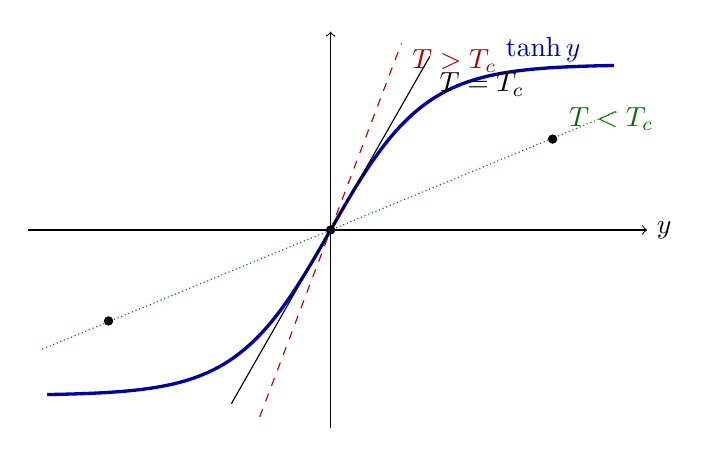
\begin{tikzpicture}[x=1.2cm,y=2.1cm]
\draw[->] (-3.2,0) -- (3.35,0) node[right] {$y$};
\draw[->] (0,-1.2) -- (0,1.2);
\draw[very thick,blue!65!black,domain=-3:3,samples=120]
  plot (\x,{tanh(\x)});
\node[blue!65!black,above] at (2.25,0.96) {$\tanh y$};
\draw[dashed,red!70!black] (-0.75,-1.13) -- (0.75,1.13);
\node[red!70!black,right] at (0.76,1.02) {$T>T_c$};
\draw[black] (-1.05,-1.05) -- (1.05,1.05);
\node[right] at (1.05,0.88) {$T=T_c$};
\draw[densely dotted,green!45!black] (-3.05,-0.72) -- (3.05,0.72);
\node[green!45!black,right] at (2.42,0.67) {$T<T_c$};
\fill (-2.35,-0.55) circle (1.7pt);
\fill (0,0) circle (1.7pt);
\fill (2.35,0.55) circle (1.7pt);
\end{tikzpicture}
\caption{Уравнение среднего поля при нулевом поле. Ниже \(T_c\) два ненулевых пересечения представляют устойчивые намагниченные фазы; нулевое решение алгебраически по-прежнему присутствует, но неустойчиво.}
\label{fig:mean-field-intersections}
\end{figure}

Поскольку
\begin{equation}
\left.\frac{d}{dy}\tanh y\right|_{y=0}=1,
\end{equation}
условие касания имеет вид
\begin{equation}
\frac{T_c}{2dJ}=1.
\end{equation}
Следовательно, приближение среднего поля предсказывает
\begin{equation}
\boxed{T_c^{\rm MF}=2dJ.}
\label{eq:sm10-mean-field-tc}
\end{equation}
Ниже этой температуры существуют два устойчивых ненулевых решения \(\pm m_0(T)\). Решение \(m=0\) по-прежнему удовлетворяет уравнению, но уже не является устойчивым равновесием. Система выбирает одну из двух связанных симметрией намагниченных фаз.

\begin{classroomqa}
\audiencequestion{Это и есть температура Кюри?}
\lecturerresponse{Да. Для ферромагнетика температуру, при которой исчезает спонтанная намагниченность, по традиции называют температурой Кюри. Здесь \(2dJ\) — ее значение в теории среднего поля, а не точный результат в низкой размерности. \lecturetimestamp{00:28:19--00:28:57}}
\end{classroomqa}

Вблизи перехода разложим гиперболический тангенс:
\begin{equation}
\tanh y=y-\frac{y^3}{3}+O(y^5).
\end{equation}
При \(h=0\) уравнение~\eqref{eq:reduced-mean-field} дает
\begin{equation}
\left(1-\frac{T}{T_c}\right)y-\frac{y^3}{3}+O(y^5)=0.
\end{equation}
Поэтому ненулевые ветви ведут себя как
\begin{equation}
y^2\simeq3\left(1-\frac{T}{T_c}\right),
\qquad
m\propto(T_c-T)^{1/2}.
\label{eq:mf-beta-exponent}
\end{equation}
Зависимость с квадратным корнем отражает критический показатель среднего поля. Его точное значение в низкой размерности не сохранится, но непрерывное обращение параметра порядка в нуль в конечной точке сохранится.

\section{Плоскость температура--поле и выбор ветви}

Материал фиксирует \(J\); экспериментатор может изменять \(T\) и \(h\). Поэтому естественно изобразить фазовую диаграмму на плоскости \(T\)--\(h\). Ниже \(T_c\) сколь угодно малое поле выбирает одну из двух намагниченных ветвей. При нашем соглашении \(h<0\) выбирает \(m>0\), тогда как \(h>0\) выбирает \(m<0\).

При нулевой температуре спины полностью выровнены, так что \(m=\pm1\). При высокой температуре среднее при нулевом поле равно \(m=0\). По мере приближения к критической точке вдоль \(h=0\) величина \(m_0(T)\) непрерывно убывает до нуля. Но при любом фиксированном \(T<T_c\) происходит скачкообразный переход от \(+m_0(T)\) к \(-m_0(T)\) при пересечении \(h=0\).

\begin{figure}[ht]
\centering
\includegraphics[width=0.90\textwidth]{lecture_10_figure_06.png}
\caption{Линия сосуществования на плоскости \(T\)--\(h\) и ветви намагниченности при фиксированной температуре ниже \(T_c\).}
\lectureframe{00:39:30}
\end{figure}

\begin{figure}[ht]
\centering
\resizebox{\linewidth}{!}{%
\begin{tikzpicture}[x=1.25cm,y=1.15cm]
\begin{scope}
\draw[->] (-2.45,0) -- (2.55,0) node[right] {$h$};
\draw[->] (0,0) -- (0,3.7) node[above] {$T$};
\draw[very thick,red!70!black] (0,0) -- (0,2.35);
\fill[red!70!black] (0,2.35) circle (2.3pt);
\node[right] at (0.08,2.35) {$T_c$};
\node at (-1.25,1.05) {$m>0$};
\node at (1.25,1.05) {$m<0$};
\draw[->,rounded corners,blue!65!black] (-1.65,0.85) -- (-1.65,3.02)
 -- (1.65,3.02) -- (1.65,0.85);
\node[blue!65!black] at (0,3.35) {continuous path};
\end{scope}
\begin{scope}[xshift=7.0cm,yshift=1.55cm]
\draw[->] (-2.5,0) -- (2.5,0) node[right] {$h$};
\draw[->] (0,-1.35) -- (0,1.4) node[above] {$m$};
\draw[very thick,blue!65!black]
  (-2.2,1.05) .. controls (-0.75,1.03) and (-0.2,0.75) .. (-0.08,0.62);
\draw[very thick,blue!65!black]
  (0.08,-0.62) .. controls (0.2,-0.75) and (0.75,-1.03) .. (2.2,-1.05);
\draw[dashed] (0,0.62) -- (0,-0.62);
\fill (0,0.62) circle (1.8pt);
\fill (0,-0.62) circle (1.8pt);
\node at (0,-1.75) {\(T<T_c\)};
\end{scope}
\end{tikzpicture}
}
\caption{При фиксированном \(T<T_c\) намагниченность скачком меняется при пересечении линии сосуществования. На полной плоскости двух параметров эти две фазы, напротив, можно соединить непрерывно, обойдя критическую точку.}
\label{fig:ising-phase-plane}
\end{figure}

\begin{classroomqa}
\audiencequestion{Что происходит, если поле в точности равно нулю ниже \(T_c\)?}
\lecturerresponse{Идеальная бесконечная система имеет две одинаково допустимые чистые фазы. Любое сколь угодно малое остаточное смещение, граничное условие или флуктуация, связанная с приготовлением, выбирает одну из них. Термодинамический разрыв выражается односторонними пределами \(m(T,0^-)=+m_0(T)\) и \(m(T,0^+)=-m_0(T)\) в нашем соглашении о знаках. \lecturetimestamp{00:35:04--00:37:10}}
\end{classroomqa}

\begin{classroomqa}
\audiencequestion{Это то же самое, что гистерезис?}
\lecturerresponse{Гистерезис связан с метастабильностью и зависящей от предыстории задержкой, с которой реальная система переключается между ветвями. Это связано, но требует динамики за пределами равновесной фазовой диаграммы и здесь не рассматривается. \lecturetimestamp{00:37:11--00:37:20}}
\end{classroomqa}

\begin{classroomqa}
\audiencequestion{Можно ли соединить положительную и отрицательную фазы, не проходя через разрыв?}
\lecturerresponse{Да. Поднимите температуру выше \(T_c\), измените там знак поля и затем снова понизьте температуру. Этот путь обходит конечную точку, и намагниченность меняется непрерывно. Скачок неизбежен только при пересечении \(h=0\) при фиксированном \(T<T_c\). \lecturetimestamp{00:37:20--00:38:15}}
\end{classroomqa}

\begin{classroomqa}
\audiencequestion{Стремится ли намагниченность к нулю всякий раз, когда \(h\) стремится к нулю?}
\lecturerresponse{Не при произвольной температуре ниже \(T_c\). Там односторонние пределы ненулевые. Самопроизвольная намагниченность стремится к нулю только при приближении к самой критической температуре. \lecturetimestamp{00:38:29--00:39:45}}
\end{classroomqa}

\section{Проницаемый ящик и химический потенциал}

Теперь оставим магниты и снова начнём с частиц. Представьте область, потенциальная энергия в которой ниже, чем в окружающем пространстве. Стенки проницаемы: частицы могут входить и выходить. Если энергия внутри ниже на величину \(\mu\), то для нахождения внутри возникает относительный множитель Больцмана \(e^{\beta\mu}\). Углубление или поднятие ямы меняет среднее число частиц в ящике.

\begin{figure}[ht]
\centering
\includegraphics[width=0.84\textwidth]{lecture_10_figure_07.png}
\caption{Картина проницаемого ящика в виде потенциальной ямы. Разность энергий между внутренней и внешней областями определяет, насколько частицы предпочитают находиться в ящике.}
\lectureframe{00:41:30}
\end{figure}

\begin{figure}[ht]
\centering
\resizebox{\linewidth}{!}{%
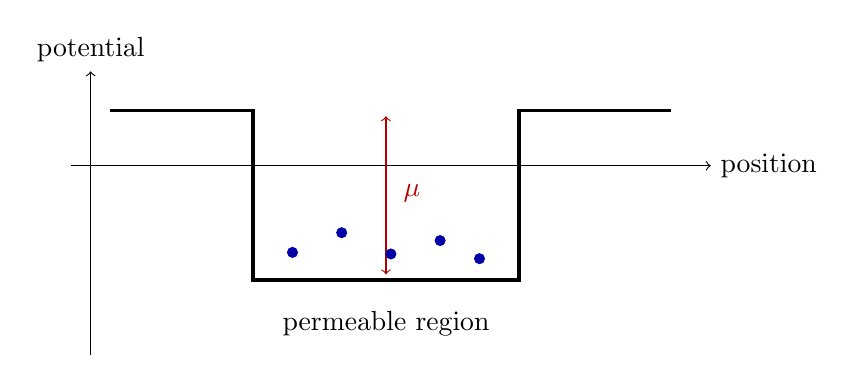
\begin{tikzpicture}[x=1.25cm,y=1.0cm]
\draw[->] (-3.2,0) -- (3.3,0) node[right] {position};
\draw[->] (-3.0,-2.4) -- (-3.0,1.2) node[above] {potential};
\draw[very thick] (-2.8,0.7) -- (-1.35,0.7)
 -- (-1.35,-1.45) -- (1.35,-1.45) -- (1.35,0.7) -- (2.9,0.7);
\draw[<->,red!70!black] (0,0.63) -- (0,-1.38);
\node[right,red!70!black] at (0.08,-0.35) {$\mu$};
\foreach \x/\y in {-0.95/-1.1,-0.45/-0.85,0.05/-1.12,0.55/-0.95,0.95/-1.18}
  \fill[blue!65!black] (\x,\y) circle (2pt);
\node at (0,-2.0) {permeable region};
\end{tikzpicture}
}
\caption{Изменение сдвига потенциала меняет предпочтительное число частиц. В большом каноническом описании этот сдвиг представляется химическим потенциалом.}
\end{figure}

Этот мысленный эксперимент делает химический потенциал наглядным. Это выигрыш в энергии на каждую добавленную частицу по сравнению с резервуаром. Если через стенку могут проходить несколько видов частиц, у каждого вида есть свой химический потенциал. Запечатанный ящик — другое дело: тогда \(N\) фиксировано, а химический потенциал определяется термодинамически, а не задаётся обменом с резервуаром.

\begin{classroomqa}
\audiencequestion{Является ли глубина ямы буквально химическим потенциалом?}
\lecturerresponse{Это прямое механическое воплощение разности химических потенциалов. Понижение каждого одночастичного уровня внутри на \(\mu\) даёт вклад \(-\mu N\) в энергию и, следовательно, \(+\beta\mu N\) в показатель Больцмана. Имеют значение только разности химического потенциала. \lecturetimestamp{00:44:49--00:45:40}}
\end{classroomqa}

Поскольку частицы могут входить и выходить, сумма по состояниям должна включать все числа частиц:
\begin{equation}
\Xi(T,\mu)
=\sum_{N=0}^{\infty}\;\sum_{\mathcal C_N}
\exp\!\left[-\beta E(\mathcal C_N)+\beta\mu N\right].
\label{eq:grand-partition}
\end{equation}
Внутренняя сумма идёт по конфигурациям при заданном \(N\); внешняя сумма — по самому \(N\). Вес большого канонического ансамбля можно также записать как \(e^{-\beta(E-\mu N)}\).

\begin{figure}[ht]
\centering
\includegraphics[width=0.88\textwidth]{lecture_10_figure_08.png}
\caption{Проницаемый ящик и большая каноническая сумма по числу частиц и конфигурациям.}
\lectureframe{00:47:15}
\end{figure}

\begin{classroomqa}
\audiencequestion{Что меняется, когда ящик запечатан?}
\lecturerresponse{Число частиц перестаёт флуктуировать. Тогда используют каноническую сумму по состояниям при фиксированном \(N\). В проницаемом ящике \(N\) является термодинамической переменной, управляемой в среднем величиной \(\mu\). \lecturetimestamp{00:45:42--00:47:50}}
\end{classroomqa}

При фиксированной температуре изменение \(\mu\) обычно плавно изменяет плотность. Ниже критической температуры оно вместо этого может вызвать резкий скачок. Это и есть искомое нами явление в жидкости. Чтобы получить его на микроскопическом уровне, частицы должны обладать двумя свойствами: они не должны иметь возможности занимать одно и то же место и должны притягиваться на малых расстояниях.

\section{Преобразование спинов в решёточный газ}

Сохраним решётку, но переинтерпретируем её два состояния. Введём число заполнения
\begin{equation}
n_i=\frac{1+\sigma_i}{2}
=
\begin{cases}
0,&\sigma_i=-1,\\
1,&\sigma_i=+1.
\end{cases}
\label{eq:occupation-map}
\end{equation}
Пустой узел соответствует спину вниз; занятый узел — спину вверх. Поскольку \(n_i\) может принимать только значения 0 или 1, двойное занятие запрещено. Следовательно, сама решётка задаёт жёсткое ядро.

\begin{figure}[ht]
\centering
\includegraphics[width=0.84\textwidth]{lecture_10_figure_04.png}
\caption{Отождествление с решёточным газом начинается с интерпретации \(\sigma=-1\) как пустого узла; тогда \(\sigma=+1\) соответствует занятому узлу.}
\lectureframe{00:53:45}
\end{figure}

Начнём с пустой решётки, где все \(\sigma=-1\). Каждая связь выровнена и имеет энергию \(-J\). Эту постоянную энергию вакуума можно вычесть. Теперь поместим одну частицу на узел двумерной решётки. Соответствующий спин переворачивается в \(+1\), разрывая четыре связи. Каждая разорванная связь стоит \(2J\), так что
\begin{equation}
\Delta E_1=4(2J)=8J.
\label{eq:one-particle-cost}
\end{equation}
Две далеко расположенные частицы разрывают восемь связей и обходятся в \(16J\). Если две частицы занимают соседние узлы, связь между ними снова оказывается выровненной. Разорваны только шесть граничных связей, и цена равна
\begin{equation}
\Delta E_{2,\rm adjacent}=6(2J)=12J.
\end{equation}
Следовательно, сближение частиц понижает энергию на
\begin{equation}
16J-12J=4J.
\label{eq:lattice-attraction}
\end{equation}
При устном подсчёте это сначала было описано как выигрыш \(2J\), а затем исправлено: одна общая связь устраняет два вклада от разорванной границы, так что притяжение равно \(4J\).

\begin{figure}[ht]
\centering
\includegraphics[width=0.84\textwidth]{lecture_10_figure_05.png}
\caption{Подсчёт связей в двух измерениях: одна изолированная частица стоит \(8J\), две далёкие частицы стоят \(16J\), а две соседние частицы стоят \(12J\).}
\lectureframe{01:00:25}
\end{figure}

У решёточного газа теперь есть оба требуемых молекулярных свойства. Двоичная занятость обеспечивает жёсткий запрет двойного занятия, а обменное взаимодействие даёт притяжение между ближайшими соседями силы \(4J\). Число частиц может флуктуировать, потому что перевороты спинов изменяют число занятых узлов.

\subsection{Точное алгебраическое соответствие}

Наглядного подсчёта связей достаточно, чтобы увидеть физику, но точная замена переменных делает эквивалентность несомненной. Подставьте
\begin{equation}
\sigma_i=2n_i-1
\end{equation}
в уравнение~\eqref{eq:ising-hamiltonian}. Для одной связи
\begin{equation}
\sigma_i\sigma_j
=4n_in_j-2n_i-2n_j+1.
\end{equation}
На регулярной \(d\)-мерной решётке
\begin{equation}
\sum_{\langle ij\rangle}(n_i+n_j)=2d\sum_i n_i.
\end{equation}
Следовательно,
\begin{align}
\mathcal H
&=-4J\sum_{\langle ij\rangle}n_in_j
+(4dJ+2h)\sum_i n_i+\text{constant}.
\label{eq:ising-as-lattice-gas}
\end{align}
Сравним это с обычным гамильтонианом решёточного газа
\begin{equation}
\mathcal H_{\rm lg}
=-\epsilon\sum_{\langle ij\rangle}n_in_j
-\mu\sum_i n_i+\text{constant}.
\label{eq:lattice-gas-hamiltonian}
\end{equation}
Соответствие имеет вид
\begin{equation}
\boxed{\epsilon=4J,\qquad
\mu=-(4dJ+2h).}
\label{eq:chemical-potential-map}
\end{equation}

\begin{figure}[ht]
\centering
\includegraphics[width=0.88\textwidth]{lecture_10_figure_09.png}
\caption{Обменный и полевой члены рядом с подсчётом энергии частиц. Поле изменяет энергию добавления частицы, не изменяя притяжения между ближайшими соседями.}
\lectureframe{01:04:30}
\end{figure}

В двух измерениях добавление изолированной частицы изменяет энергию на
\begin{equation}
8J+2h=-\mu.
\end{equation}
Член \(8J\) возникает из-за разорванных связей; член \(2h\) — из-за изменения одного спина с \(-1\) на \(+1\). Поэтому, изменяя \(h\), мы изменяем химический потенциал, оставляя притяжение \(4J\) фиксированным. Поле не равно буквально \(\mu\), поскольку обменный фон вносит сдвиг \(4dJ\).

\begin{classroomqa}
\audiencequestion{Если поле управляет числом частиц, почему \(h\) не является просто химическим потенциалом?}
\lecturerresponse{Создание частицы также разрывает обменные связи относительно пустого опорного состояния. Поэтому обычный коэффициент при \(-N\) равен \(\mu=-(4dJ+2h)\), а не просто \(-2h\). Сдвиг зависит от \(J\) и координационного числа. \lecturetimestamp{01:06:28--01:06:41}}
\end{classroomqa}

Плотность столь же проста:
\begin{equation}
\rho=\expect{n_i}
=\frac{1+\expect{\sigma_i}}{2}
=\frac{1+m}{2}.
\label{eq:density-map}
\end{equation}
Тем самым \(m=-1\) соответствует пустой решётке, \(m=+1\) — полностью заполненной решётке, а \(m=0\) — половинному заполнению. Полное число частиц равно \(N_{\rm p}=\sum_i n_i\); плотность равна \(N_{\rm p}/N\).

\begin{figure}[ht]
\centering
\includegraphics[width=0.90\textwidth]{lecture_10_figure_10.png}
\caption{Соотношение для плотности \(\rho=(1+m)/2\), записанное рядом с линией магнитного сосуществования.}
\lectureframe{01:08:25}
\end{figure}

\begin{classroomqa}
\audiencequestion{Является ли \((1+m)/2\) числом частиц или плотностью?}
\lecturerresponse{Это средняя заселённость на узел, то есть безразмерная решёточная плотность. Умножение на полное число узлов даёт ожидаемое число частиц. Различие между интенсивной плотностью и экстенсивным числом важно. \lecturetimestamp{01:06:43--01:09:31}}
\end{classroomqa}

\section{Магнитная фазовая диаграмма становится фазовой диаграммой флюида}

Переведём рисунок~\ref{fig:ising-phase-plane} с помощью уравнений~\eqref{eq:chemical-potential-map} и \eqref{eq:density-map}. Выше \(T_c\) изменение \(\mu\) плавно меняет плотность. Ниже \(T_c\) пересечение значения сосуществования
\begin{equation}
\mu_{\rm coex}=-4dJ
\qquad(h=0)
\label{eq:coexistence-mu}
\end{equation}
вызывает скачок плотности между разреженным газом и плотной жидкостью. При \(T_c\) эти две плотности сливаются, и разрыв исчезает.

\begin{figure}[ht]
\centering
\includegraphics[width=0.92\textwidth]{lecture_10_figure_11.png}
\caption{Линия сосуществования Изинга, рассматриваемая как фазовая диаграмма жидкость--газ. Газ находится со стороны малой плотности, жидкость — со стороны большой плотности, и их можно непрерывно соединить, обойдя критическую конечную точку.}
\lectureframe{01:14:30}
\end{figure}

\begin{figure}[ht]
\centering
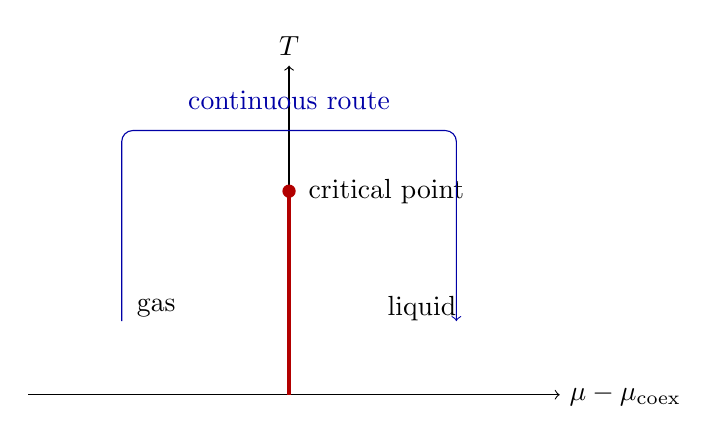
\begin{tikzpicture}[x=1.25cm,y=1.1cm]
\draw[->] (-2.65,0) -- (2.75,0) node[right] {$\mu-\mu_{\rm coex}$};
\draw[->] (0,0) -- (0,3.8) node[above] {$T$};
\draw[very thick,red!70!black] (0,0) -- (0,2.35);
\fill[red!70!black] (0,2.35) circle (2.4pt);
\node[right] at (0.1,2.35) {critical point};
\node at (-1.35,1.0) {gas};
\node at (1.35,1.0) {liquid};
\draw[->,blue!65!black,rounded corners]
 (-1.7,0.85) -- (-1.7,3.05) -- (1.7,3.05) -- (1.7,0.85);
\node[blue!65!black] at (0,3.4) {continuous route};
\end{tikzpicture}
\caption{Ниже конечной точки жидкость и газ — различные фазы, однако в сверхкритической области между ними нет сингулярной границы.}
\label{fig:liquid-gas-plane}
\end{figure}

Это и есть знакомая линия кипения. При фиксированном давлении нагревание жидкости до пересечения линии сосуществования приводит к кипению. При фиксированной температуре ту же границу можно пересечь, изменяя давление или химический потенциал. Перегретый пар или переохлаждённая жидкость — метастабильное продолжение за пределами равновесного сосуществования; описание времени жизни такого состояния требует динамики нуклеации, которая выходит за рамки этой равновесной конструкции.

\begin{classroomqa}
\audiencequestion{Представлен ли на этой фазовой диаграмме перегретый пар?}
\lecturerresponse{Равновесная диаграмма задаёт границу сосуществования. Перегретое или пересыщенное состояние метастабильно: оно временно сохраняется по неправильную сторону границы, потому что образование критической капли связано с затратой свободной энергии на границе раздела. Это кинетическое уточнение здесь не вычисляется. \lecturetimestamp{01:12:19--01:12:29}}
\end{classroomqa}

\begin{classroomqa}
\audiencequestion{Как изменяют химический потенциал в обычном флюиде?}
\lecturerresponse{Ящик с потенциальной ямой — это чистый теоретический способ управления. В лаборатории чаще изменяют давление, объём или контакт с резервуаром; затем термодинамика переводит эти управляющие параметры в изменение химического потенциала. \lecturetimestamp{01:12:30--01:13:59}}
\end{classroomqa}

\begin{classroomqa}
\audiencequestion{Когда меняется плотность, изменяем ли мы молекулярный потенциал \(J\)?}
\lecturerresponse{Нет. Для фиксированного вещества \(J\) представляет короткодействующее притяжение и в этой модели остаётся фиксированным. Изменение \(\mu\) меняет, сколько узлов занято, и тем самым распределение межмолекулярных расстояний. Изменение \(J\) означало бы изменение микроскопического вещества или взаимодействия. \lecturetimestamp{01:14:50--01:15:41}}
\end{classroomqa}

\begin{classroomqa}
\audiencequestion{Совпадает ли критическая температура с обычной температурой кипения?}
\lecturerresponse{Нет. Температура кипения задаётся при выбранном давлении, поэтому при изменении давления она перемещается вдоль кривой сосуществования. Критическая температура — это единственная конечная точка, выше которой жидкость и газ больше не разделены фазовой границей. В этом рассмотрении решёточного газа давление явно не выводилось. \lecturetimestamp{01:15:42--01:17:02}}
\end{classroomqa}

Теперь можно сформулировать центральный результат. Магнетик Изинга и решёточный газ не просто дают похожие диаграммы. После замены переменных и параметров у них одна и та же статистическая сумма. Каждому сингулярному термодинамическому свойству на одной стороне соответствует аналог на другой:
\begin{equation}
\begin{array}{c|c}
\text{Ising magnet} & \text{lattice gas}\\ \hline
\sigma_i=\pm1 & n_i=0,1\\
m=\expect{\sigma} & \rho=(1+m)/2\\
h & \mu=-(4dJ+2h)\\
\text{aligned exchange} & \text{nearest-neighbor attraction}\\
h=0,\ T<T_c & \text{liquid--gas coexistence}\\
(T_c,0) & \text{critical endpoint}
\end{array}
\label{eq:ising-fluid-dictionary}
\end{equation}

\section{Критические показатели и универсальность}

Вблизи критической точки термодинамические величины часто приобретают степенные сингулярности. Вводя приведённую температуру
\begin{equation}
t=\frac{T-T_c}{T_c},
\end{equation}
схематически пишут,
\begin{equation}
m\sim(-t)^{\beta_{\rm crit}},
\qquad
\chi\sim |t|^{-\gamma},
\qquad
\xi\sim |t|^{-\nu}.
\label{eq:critical-exponents}
\end{equation}
Здесь \(\beta_{\rm crit}\) — критический показатель, а не обратная температура. Теория среднего поля даёт \(\beta_{\rm crit}=1/2\), но ниже верхней критической размерности флуктуации изменяют показатели.

Показатели не обязаны быть целыми. Не обязаны они и все быть иррациональными: у двумерной модели Изинга, как хорошо известно, есть несколько точных рациональных показателей, тогда как трёхмерные значения для Изинга — нетривиальные числа, определённые с высокой точностью теорией и вычислениями. Надёжный вывод состоит в том, что эти показатели вообще говоря не определяются элементарным анализом размерностей.

Ещё поразительнее то, что микроскопические детали часто не фиксируют их. Системы с одной и той же пространственной размерностью, одной и той же симметрией параметра порядка и достаточно короткодействующими взаимодействиями могут приходить к одной и той же критической теории на больших расстояниях. Они принадлежат к одному \emph{классу универсальности}. Одноосный магнетик и обычная конечная точка жидкость--газ оба имеют один скалярный параметр порядка и в одной и той же размерности принадлежат к классу универсальности Изинга.

\begin{classroomqa}
\audiencequestion{Составляют ли классы универсальности конечный или дискретный список?}
\lecturerresponse{Классов много; они организуются по размерности, симметриям, законам сохранения, дальности взаимодействия и другим крупномасштабным характеристикам. Во многих знакомых случаях неподвижные точки и наборы показателей дискретны, но существуют и системы с непрерывно меняющимися показателями. Надёжное утверждение состоит не в том, что каталог конечен, а в том, что многие микроскопически разные системы имеют одни и те же крупномасштабные характеристики. \lecturetimestamp{01:18:50--01:19:38}}
\end{classroomqa}

\begin{classroomqa}
\audiencequestion{Если жидкость и газ сосуществуют, что разделяет их в реальном сосуде?}
\lecturerresponse{Граница раздела. Поверхностное натяжение делает площадь этой границы энергетически невыгодной, а гравитация создаёт вертикальный градиент химического потенциала и обычно располагает более плотную жидкость ниже газа. При пренебрежимо малой гравитации геометрия более непосредственно определяется поверхностным натяжением и граничными условиями. \lecturetimestamp{01:19:40--01:21:18}}
\end{classroomqa}

\begin{classroomqa}
\audiencequestion{Где в этой картине теплота парообразования?}
\lecturerresponse{Ниже критической точки пересечение линии сосуществования первого рода обычно сопровождается скрытой теплотой. Теплота парообразования стремится к нулю при приближении к критической конечной точке, потому что там две фазы становятся тождественными. Эта лекция устанавливает фазовую структуру, но не вычисляет скрытую теплоту. \lecturetimestamp{01:21:19--01:22:18}}
\end{classroomqa}

\begin{classroomqa}
\audiencequestion{Можно ли использовать фазовый переход как чувствительный детектор, например в сверхпроводящем устройстве?}
\lecturerresponse{Да. Вблизи перехода малое возмущение может вызвать большой отклик или запустить смену состояния. Практические детекторы используют эту чувствительность, хотя соответствующие параметр порядка и динамика могут отличаться от примера Изинга. \lecturetimestamp{01:22:19--01:24:05}}
\end{classroomqa}

Этим курс статистической механики завершается. Путь начался с энтропии и равновесия, прошёл через статистические суммы и газы и завершился демонстрацией того, что магнетик и флюид могут быть двумя описаниями одного и того же критического явления.

\section{Послелекционная дискуссия: тонкая настройка и отбор}

После окончания формальной лекции разговор продолжался ещё примерно 40 минут. Его стоит сохранить, но не следует путать с приведённым выше выводом. Предметом теперь уже не является решёточный газ. Речь идёт о логике тонкой настройки и об осторожном использовании антропного отбора в космологии.

\subsection{Малые числа сами по себе не означают тонкой настройки}

Не существует одной фразы, которая окончательно проясняла бы всякое употребление выражения \emph{антропный принцип}. Полезная отправная точка — операциональная: когда теория допускает много реализованных сред, наблюдения обусловлены тем фактом, что наблюдатели могут возникнуть лишь в некоторых из них. Такое условное утверждение может быть разумным. Оно становится пустым, если ссылаться на него без ансамбля, условия отбора или механизма, делающего альтернативы физически осмысленными.

Прежде чем вводить отбор, нужно отличать малый параметр от тонко настроенного. Число может быть малым, потому что устойчивый динамический механизм приводит его к особому значению. Тонкая настройка означает, что наблюдаемое значение, по-видимому, требует чрезвычайно точного баланса между в остальном независимыми вкладами, причём не известны ни восстанавливающий механизм, ни симметрия, защищающая этот баланс.

\begin{classroomqa}
\audiencequestion{Можно ли сформулировать антропный принцип в строгой форме?}
\lecturerresponse{Его оправданное применение условно, а не мистично: если многие физически реализованные среды имеют разные параметры, то среды, наблюдаемые такими существами, как мы, выбираются из подмножества, совместимого с существованием наблюдателей. Это само по себе не порождает эти среды и не назначает им вероятности; эти задачи относятся к лежащей в основе физике. \lecturetimestamp{01:25:45--01:26:13}}
\end{classroomqa}

Космологическая постоянная — мотивирующий пример. Ее наблюдаемая величина чрезвычайно мала по сравнению с наивными вкладами квантовой теории поля в энергию вакуума. Трудность состоит не просто в том, что итоговое число мало. Она в том, что, по-видимому, многие большие члены должны сокращаться с колоссальной точностью, тогда как никакого общепринятого низкоэнергетического механизма обратной связи, подстраивающего результат к наблюдаемому значению, не существует.

\subsection{Дирижабль и подводная лодка}

Два примера плавучести выявляют это различие. Дирижабль парит на такой высоте, где его средняя плотность совпадает с плотностью окружающего воздуха. Плотность воздуха уменьшается с высотой. Если дирижабль поднимается, внешний воздух становится менее плотным, и дирижабль стремится опуститься; если он опускается, внешний воздух становится более плотным, и дирижабль стремится подняться. Совпадение плотностей может быть численно тонким, но атмосферный градиент обеспечивает восстанавливающую обратную связь. Равновесие объясняется динамически.

Нейтрально плавучая подводная лодка в почти несжимаемой воде — иной случай. Плотность воды мало меняется с глубиной. Если средняя плотность подводной лодки случайно равна плотности окружающей воды, никакой сопоставимый зависящий от глубины восстанавливающий механизм не объясняет это равенство. Крошечное несовпадение заставляет ее всплывать или тонуть. Для достижения нейтральной плавучести нужна точная регулировка балласта и содержимого. Тогда малый остаток представляет собой тонкую настройку, если только его не объясняет какая-то система управления или конструктивный механизм.

\begin{figure}[ht]
\centering
\resizebox{\linewidth}{!}{%
\begin{tikzpicture}[>=Latex]
\begin{scope}[xshift=-3.8cm]
\shade[top color=blue!5,bottom color=blue!28] (-2.5,-2.2) rectangle (2.5,2.2);
\draw[very thick,rounded corners=18pt,fill=yellow!35]
  (-1.15,0) ellipse (1.15 and 0.55);
\draw[thick] (0,-0.55) -- (0,-1.05);
\draw[thick,fill=gray!20] (-0.45,-1.05) rectangle (0.45,-1.38);
\draw[->,red!70!black,thick] (1.65,1.45) -- (1.65,0.55)
 node[midway,right] {restoring};
\draw[->,red!70!black,thick] (-1.65,-1.45) -- (-1.65,-0.55)
 node[midway,left] {restoring};
\node at (0,2.55) {\textbf{Blimp: density gradient}};
\node[align=center] at (0,-2.75) {displacement changes\\the buoyant imbalance};
\end{scope}
\begin{scope}[xshift=3.8cm]
\shade[top color=cyan!10,bottom color=blue!45] (-2.5,-2.2) rectangle (2.5,2.2);
\draw[very thick,fill=gray!35,rounded corners=12pt]
  (-1.45,-0.25) -- (1.1,-0.25) arc (-90:90:0.38)
  -- (-1.45,0.51) -- cycle;
\draw[thick] (-0.25,0.51) -- (-0.25,0.85) -- (0.35,0.85) -- (0.35,0.51);
\draw[->,red!70!black,thick] (1.65,0.15) -- (1.65,1.35)
 node[midway,right] {rise};
\draw[->,red!70!black,thick] (-1.65,0.15) -- (-1.65,-1.35)
 node[midway,left] {sink};
\node at (0,2.55) {\textbf{Submarine: nearly uniform density}};
\node[align=center] at (0,-2.75) {no depth-dependent feedback\\protects neutral buoyancy};
\end{scope}
\end{tikzpicture}
}
\caption{Малый остаток может быть динамически устойчивым или действительно требовать тонкой настройки. У дирижабля есть восстанавливающая обратная связь; для идеализированной подводной лодки необходимо подогнать ее среднюю плотность к плотности воды.}
\label{fig:blimp-submarine}
\end{figure}

\begin{classroomqa}
\audiencequestion{Почему экипаж подводной лодки должен требовать объяснения, если наблюдается нейтральная плавучесть?}
\lecturerresponse{Потому что при отсутствии механизма управления балластом ни симметрия, ни обратная связь со средой не защищают равенство двух независимых плотностей. Вопрос не в том, логически ли возможно это равенство, а в том, почему система находится в столь узкой области своего пространства параметров. \lecturetimestamp{01:35:05--01:36:25}}
\end{classroomqa}

\subsection{Многие области и обусловленность наблюдений}

Теперь представим процесс, который порождает огромное число подводных лодок со многими разными средними плотностями. Большинство тонет или всплывает; лишь ничтожная доля надолго остается в обитаемой полосе между поверхностью и дном. Наблюдатель, который по необходимости живет в одной из сохранившихся подводных лодок, не должен удивляться, измерив почти нейтральную плавучесть. Наблюдение отбирается условием, необходимым для присутствия наблюдателя.

Для такого рассуждения нужны две составляющие:
\begin{enumerate}
\item физический процесс, который действительно реализует много альтернатив, а не альтернативы, существующие лишь в воображении;
\item условие отбора, объясняющее, почему наблюдения возможны только в ограниченном подмножестве.
\end{enumerate}
Отбор не заменяет механизм порождения. Он меняет условную вероятность того, что измерит наблюдатель, когда ансамбль уже существует.

\begin{classroomqa}
\audiencequestion{Сводится ли этот аргумент просто к тому, что в достаточно большой выборке где-то происходят маловероятные события?}
\lecturerresponse{Это лишь первая половина. Вторая — обусловленность наблюдений: наблюдатели выбираются не равномерно из всех областей, а только из тех, где их существование возможно. Чтобы предложение было полноценным, все равно нужны мера на пространстве областей и физическое описание того, как они порождаются. \lecturetimestamp{01:39:19--01:40:36}}
\end{classroomqa}

Применительно к энергии вакуума большая отрицательная космологическая постоянная может заставить вселенную слишком быстро вновь схлопнуться, тогда как достаточно большое положительное значение может помешать веществу сконденсироваться в галактики. Наблюдаемое значение лежит в узком диапазоне, совместимом с долгоживущими структурами. Это дает возможное условие отбора, а не вывод распределения значений космологической постоянной.

Квантовая теория поля добавляет проблему тонкой настройки: вакуумные вклады от разных полей и масштабов по отдельности намного больше наблюдаемого остатка. Если эти члены почти в точности сокращаются, результат больше напоминает тщательно уравновешенную подводную лодку, чем самокорректирующийся дирижабль. Аналогия призвана выявить логическую проблему, а не дать ее решение.

\begin{classroomqa}
\audiencequestion{Могут ли изменения одного параметра компенсироваться изменениями нескольких других?}
\lecturerresponse{Да. Допустимое множество не обязано быть узким интервалом на одной оси; оно может быть тонкой поверхностью в многомерном пространстве параметров. Коррелированные изменения могут сохранять структуру, но тогда вопрос сводится к тому, почему реализованные параметры лежат вблизи этой поверхности и какую меру приписывает ей лежащая в основе теория. \lecturetimestamp{01:45:10--01:46:19}}
\end{classroomqa}

\begin{figure}[ht]
\centering
\begin{tikzpicture}[x=1.3cm,y=1.05cm,>=Latex]
\draw[->] (-3.2,0) -- (3.4,0) node[right] {$\lambda_1$};
\draw[->] (0,-2.5) -- (0,2.65) node[above] {$\lambda_2$};
\fill[gray!12] (-3,-2.25) rectangle (3.1,2.3);
\draw[very thick,blue!65!black]
 (-2.8,-1.55) .. controls (-1.3,-0.75) and (0.15,0.05) .. (2.85,1.55);
\draw[very thick,blue!25]
 (-2.8,-1.25) .. controls (-1.3,-0.45) and (0.15,0.35) .. (2.85,1.85);
\fill[blue!15,opacity=.65]
 (-2.8,-1.55) .. controls (-1.3,-0.75) and (0.15,0.05) .. (2.85,1.55)
 -- (2.85,1.85) .. controls (0.15,0.35) and (-1.3,-0.45) .. (-2.8,-1.25) -- cycle;
\node[blue!65!black,rotate=28] at (1.3,0.95) {viable band};
\foreach \x/\y in {-2.4/1.45,-1.7/-1.8,-0.9/1.8,0.3/-1.45,1.2/1.85,2.4/-0.8}
  \fill[red!65!black] (\x,\y) circle (2pt);
\fill[green!45!black] (0.55,0.58) circle (2.8pt);
\node[green!35!black,right] at (0.65,0.55) {observed domain};
\end{tikzpicture}
\caption{При нескольких параметрах обитаемость или возможность существования структур может занимать тонкую коррелированную полосу, а не узкий интервал одного параметра. Отбор ограничивает наблюдения этой полосой, но не порождает распределение параметров.}
\label{fig:viable-parameter-band}
\end{figure}

\subsection{Ландшафтные сценарии и их неопределенности}

Одним из предложенных источников альтернатив является теория со многими метастабильными вакуумами, возможно реализуемыми в разных космологических областях. Идеи ландшафта теории струн и сценарии вечной инфляции — примеры, но их детальная реализация и вероятностная мера остаются неопределенными. В лекции это представлено как возможность, а не как установленный факт.

Симметрия была бы более привычным объяснением, если бы она заставляла космологическую постоянную обращаться точно в нуль. Трудность в том, что наблюдаемое ускоренное расширение соответствует малому ненулевому значению. Механизм, который естественным образом дает в точности нуль, сам по себе не объясняет крошечный остаток; нарушение симметрии может просто вновь ввести тонкую настройку. Здесь вновь возвращается образ подводной лодки: трос мог бы удерживать ее на выбранной глубине, но тогда именно он и есть механизм, который нужно указать, а не просто предположить.

\begin{classroomqa}
\audiencequestion{Нарушает ли очень точное измерение параметра принцип неопределенности?}
\lecturerresponse{Нет. Соотношение неопределенностей относится к заданным парам некоммутирующих наблюдаемых. Константа связи или вакуумный параметр может иметь резко определенное значение, не будучи канонически сопряженным с неконтролируемой наблюдаемой. Сама по себе точность не является парадоксом принципа неопределенности. \lecturetimestamp{01:49:21--01:49:36}}
\end{classroomqa}

\begin{classroomqa}
\audiencequestion{Объясняет ли антропное рассуждение значение, или лишь переформулирует, что оно необходимо наблюдателям?}
\lecturerresponse{Сам по себе отбор не является динамическим объяснением. Его правомерная роль состоит в изменении условных вероятностей в физически реализованном ансамбле. Если пользоваться им без ансамбля, меры или проверяемых следствий, он рискует стать скорее ярлыком, чем объяснением. \lecturetimestamp{01:49:37--01:50:21}}
\end{classroomqa}

\subsection{Умеренные совпадения в физике частиц}

Не каждый существенный для жизни параметр настроен в одинаково чрезвычайной степени. Обычное вещество зависит от фотонов, электронов, легких кварков и сильного взаимодействия; нейтрино влияют на космологию, но не являются непосредственными агентами, связывающими атомы. Разность масс протона--нейтрона особенно важна. Поскольку нейтрон немного тяжелее протона, изолированные нейтроны могут распадаться, а обычный водород стабилен. Если бы их порядок был достаточно сильно обращен, ядерная химия радикально изменилась бы.

Масса электрона и постоянная тонкой структуры аналогичным образом задают атомные размеры и энергии связи. Их существенное изменение изменило бы химию. Это содержательные утверждения о чувствительности, но их не следует раздувать до утверждения, будто любое малое изменение исключает любую мыслимую форму сложности. По сравнению с проблемой космологической постоянной многие такие совпадения умеренны и коррелированы с другими параметрами.

Иерархия, связанная с электрослабым масштабом, — еще одна заметная проблема естественности: радиационные вклады, как правило, делают массу фундаментального скаляра чувствительной к высоким масштабам, если ее не защищает дополнительная структура. Ее статус и интерпретация отличаются от проблемы энергии вакуума, и ни одну из них не следует сводить к лозунгу.

\begin{classroomqa}
\audiencequestion{Действительно ли изменение разности масс протона--нейтрона имело бы значение для обычного вещества?}
\lecturerresponse{Да. Наблюдаемый порядок допускает стабильный водород и определяет бета-стабильность различных ядер. Умеренные изменения могут перестроить ядерные распространенности и горение в звездах. В тщательном анализе нужно согласованно варьировать связанные параметры, а не менять одно число, оставляя все остальные фиксированными. \lecturetimestamp{01:51:47--01:53:08}}
\end{classroomqa}

\begin{classroomqa}
\audiencequestion{Какую роль играют масса электрона и постоянная тонкой структуры?}
\lecturerresponse{Они задают характерные атомные масштабы энергии и длины, схематически \(E_{\rm atom}\sim \alpha^2m_e\) и \(a_0\sim(\alpha m_e)^{-1}\) в единицах \(\hbar=c=1\). Большие изменения изменили бы химию, хотя точная область допустимых значений — многомерный вопрос. \lecturetimestamp{01:53:09--01:54:12}}
\end{classroomqa}

\subsection{Разногласия, временная зависимость и проверки}

Обсуждение ненадолго обращается к критике инфляции и к интерпретации высокоточных космологических данных. Это историческое разногласие следует представлять именно как разногласие, а не считать разрешённым риторикой. У инфляции есть успешные феноменологические предсказания и множество вариантов моделей; вопросы о начальных условиях, мерах и проверяемости остаются активной областью исследований. Данные накладывают ограничения на модели, но ни одна отдельная ссылка в разговоре на какой-либо эксперимент не решает вопрос обо всей этой схеме.

\begin{classroomqa}
\audiencequestion{Могла ли космологическая постоянная медленно меняться со временем, вместо того чтобы оставаться постоянной?}
\lecturerresponse{Динамическое поле тёмной энергии может приводить к зависящему от времени ускорению. Оно вводит потенциал и начальные условия, которые сами требуют объяснения, а наблюдения ограничивают уравнение состояния так, что оно должно быть близким к случаю космологической постоянной. В обсуждении на момент лекции никакие данные не требовали заметной временной зависимости. \lecturetimestamp{01:57:17--01:59:19}}
\end{classroomqa}

\begin{classroomqa}
\audiencequestion{Вызывает ли сам антропный отбор нуклеацию разных вселенных или доменов?}
\lecturerresponse{Нет. Отбор указывает, какие из реализованных доменов могут содержать наблюдателей; он не создаёт сами домены. Их должен был бы порождать отдельный космологический механизм, например вакуумные переходы в ходе инфляционной истории. \lecturetimestamp{01:59:20--01:59:42}}
\end{classroomqa}

Причинный порядок должен оставаться ясным:
\begin{equation}
\begin{gathered}
\text{laws and initial conditions}\\[-0.15em]
\downarrow\\[-0.15em]
\text{physical environments}\\[-0.15em]
\downarrow\\[-0.15em]
\text{observers and observations}
\end{gathered}
\end{equation}
Наблюдатели не воздействуют назад и не диктуют законы. Условление появляется тогда, когда мы спрашиваем, что, вероятно, измерит наблюдатель, выбранный из реализованных сред.

Поэтому научный вопрос состоит не в том, звучит ли эта терминология философски, политически или религиозно. Он состоит в том, имеет ли это предложение определённый физический ансамбль, вычислимую или по крайней мере ограниченную меру и следствия, которые могли бы отличить его от альтернатив. К возможным признакам, обсуждавшимся для многовакуумной космологии, относятся следы столкновений между пузырьковыми доменами. Такие сигналы трудно надёжно предсказывать, и в обсуждении на момент лекции ни один из них не был установлен в космическом микроволновом фоне. Отсутствие простого теста — серьёзное ограничение, а не основание ни объявлять эту идею истинной, ни отмахиваться от самой проблемы тонкой настройки.

\begin{classroomqa}
\audiencequestion{Что превратило бы это из аргумента, основанного на отборе, в научную теорию?}
\lecturerresponse{Этому предложению нужны механизм, который порождает альтернативы, вероятностная мера или контролируемый её заменитель, и наблюдаемые следствия. Сигнатуры столкновений пузырей — один из возможных путей, но их отсутствие или неоднозначность показывает, насколько трудна проблема проверяемости. \lecturetimestamp{02:02:31--02:04:12}}
\end{classroomqa}

Послелекционная дискуссия завершается на этой методологически строгой ноте. Тонкая настройка — свидетельство того, что какого-то объяснения, возможно, недостаёт. Симметрия, динамическая подстройка и средовой отбор — логически различные возможные объяснения. Такой подход может быть рационален, но лишь как один из компонентов физического описания, предпосылки и пределы которого сформулированы открыто.
